\documentclass[12pt]{article}

\usepackage{amsmath}
\usepackage{amssymb}
\usepackage{graphicx}
\usepackage{hyperref}
\usepackage{natbib}
\usepackage{booktabs}
\usepackage[margin=1in]{geometry}
\usepackage{xcolor}

\bibliographystyle{aasjournal}

\title{HII Region Expansion: From Ionization Balance\\to the Modified Spitzer Solution}
\author{Chang-Goo Kim}
\date{\today}

\begin{document}
\maketitle

\begin{abstract}
We present a self-contained derivation of the physics governing the expansion
of HII regions around young OB stars, from ionization balance through the
Str\"omgren sphere and the classic Spitzer thin-shell solution, to a modified
formulation that correctly accounts for the shell mass physics.  The analytic
and numerical results are implemented in the open-source Python package
\texttt{hii-expansion}, which integrates the thin-shell momentum equation in CGS
units using \texttt{scipy} and \texttt{astropy}.
\end{abstract}

%-----------------------------------------------------------------------
\section{Introduction}
\label{sec:intro}
%-----------------------------------------------------------------------

Young massive OB stars emit copious ionizing photons ($h\nu > 13.6$ eV),
carving out ionized nebulae---HII regions---in the surrounding interstellar
medium.  The rapid pressurization of the ionized gas drives a thin neutral
shell outward, sweeping up ambient material in a process that shapes the
structure of star-forming molecular clouds and regulates the efficiency of
subsequent star formation.  This note develops the physics of HII region
expansion from first principles, beginning with ionization balance and the
Str\"omgren sphere concept \citep{Stromgren1939}, proceeding through the
dynamical thin-shell model of \citet{Spitzer1978}, and concluding with a
modified formulation that corrects the treatment of the shell mass.
All calculations are performed in CGS units using the Python package
\texttt{hii-expansion} built on \texttt{scipy} \citep{Virtanen2020} and
\texttt{astropy} \citep{Astropy2022}.

%-----------------------------------------------------------------------
\section{Ionization and Recombination Balance}
\label{sec:ionization}
%-----------------------------------------------------------------------

In the interior of an HII region the gas is fully photoionized by the central
star.  In steady state the ionizing photon rate $Q$ (photons s$^{-1}$) equals
the total recombination rate within the ionized volume:
\begin{equation}
  \label{eq:ionbal}
  Q = 4\pi\alpha_B \int_0^{R} n(r)^2\, r^2\, dr,
\end{equation}
where $n(r)$ is the hydrogen number density and $\alpha_B$ is the case B
recombination coefficient, which accounts for recombinations to all levels
except the ground state \citep{OsterbrockFerland2006}.

\subsection{Case B recombination coefficient}

We use the fitting formula of \citet{Draine2011}:
\begin{equation}
  \label{eq:alphaB}
  \alpha_B(T) = 2.54\times10^{-13}\, t_4^{-0.8163 - 0.0208\ln t_4}
                \quad \mathrm{cm}^3\,\mathrm{s}^{-1},
                \qquad t_4 \equiv \frac{T}{10^4\,\mathrm{K}},
\end{equation}
valid for $3\,000 \le T \le 30\,000$ K \citep{StoreyHummer1995}.  At
$T=10^4$ K, $\alpha_B \approx 2.54\times10^{-13}$ cm$^3$ s$^{-1}$.

\subsection{Effective ionized density}

Assuming that the ionization front propagates quasi-statically so that
Equation~(\ref{eq:ionbal}) is satisfied instantaneously, the mean ionized
density within radius $R$ is
\begin{equation}
  \label{eq:ni}
  n_i(R) = \sqrt{\frac{3Q}{4\pi\alpha_B R^3}} \propto R^{-3/2}.
\end{equation}
This quantity sets the interior gas pressure (Section~\ref{sec:spitzer}).

%-----------------------------------------------------------------------
\section{The Str\"omgren Sphere}
\label{sec:stromgren}
%-----------------------------------------------------------------------

\subsection{Uniform density}

For a uniform ambient density $n$, Equation~(\ref{eq:ionbal}) gives an exact
analytic result for the Str\"omgren radius:
\begin{equation}
  \label{eq:Rst_uniform}
  R_\mathrm{st} = \left(\frac{3Q}{4\pi n^2 \alpha_B}\right)^{1/3}.
\end{equation}
This scales as $R_\mathrm{st}\propto Q^{1/3} n^{-2/3} \alpha_B^{-1/3}$.
For fiducial parameters $Q=10^{49}$ s$^{-1}$, $n_0=100$ cm$^{-3}$,
$T=10^4$ K, Equation~(\ref{eq:Rst_uniform}) yields
$R_\mathrm{st}\approx 3.18$ pc.

\subsection{Arbitrary density profile}

For a radial density profile $n(r)$ the Str\"omgren radius is found
numerically by root-finding on
\begin{equation}
  \label{eq:Rst_numeric}
  f(R) = 4\pi\alpha_B\int_0^R n(r)^2 r^2\, dr - Q = 0
\end{equation}
using Brent's method, with the bracket expanded geometrically until
$f(r_\mathrm{hi}) \ge 0$.

The effective rms density at the Str\"omgren radius is
\begin{equation}
  \label{eq:nrms}
  n_\mathrm{rms} = \sqrt{\frac{3Q}{4\pi\alpha_B R_\mathrm{st}^3}},
\end{equation}
which equals $n_0$ for uniform density and is reduced for declining profiles.
If $4\pi\alpha_B\int_0^\infty n^2 r^2\, dr < Q$ the medium is
\emph{density-bounded}: all ambient photons are used for ionization even at
infinite radius and no finite Str\"omgren sphere exists.

\subsection{Cored density profiles}

Table~\ref{tab:cored} reports $R_\mathrm{st}$ and $n_\mathrm{rms}$ for the
cored profile
\begin{equation}
  n(r) = \frac{n_0}{1+(r/r_0)^w}
\end{equation}
with $r_0\in\{1,5,10\}$ pc and $w\in\{1,1.5,2\}$.  The $r_0=1$ pc,
$w\ge 1.5$ cases are density-bounded.

\begin{table}[ht]
\centering
\caption{Str\"omgren radius and rms density for cored profiles.
         Parameters: $Q=10^{49}$ s$^{-1}$, $n_0=100$ cm$^{-3}$,
         $T=10^4$ K. ``DB'' = density-bounded.}
\label{tab:cored}
\begin{tabular}{rrrrr}
\toprule
$r_0$ [pc] & $w$ & $R_\mathrm{st}$ [pc] & $n_\mathrm{rms}$ [cm$^{-3}$] & $n_\mathrm{rms}/n_0$ \\
\midrule
0 (uniform) & --- & 3.175 & 100.0 & 1.0000 \\
\midrule
1  & 1.0 & 15.308 &  9.44 & 0.0944 \\
1  & 1.5 & \multicolumn{3}{c}{DB} \\
1  & 2.0 & \multicolumn{3}{c}{DB} \\
\midrule
5  & 1.0 &  4.395 & 61.39 & 0.6139 \\
5  & 1.5 &  4.081 & 68.60 & 0.6860 \\
5  & 2.0 &  3.827 & 75.55 & 0.7555 \\
\midrule
10 & 1.0 &  3.729 & 78.55 & 0.7855 \\
10 & 1.5 &  3.448 & 88.35 & 0.8835 \\
10 & 2.0 &  3.310 & 93.94 & 0.9394 \\
\bottomrule
\end{tabular}
\end{table}

%-----------------------------------------------------------------------
\section{Thin-Shell Momentum Equation: Classic Spitzer Solution}
\label{sec:spitzer}
%-----------------------------------------------------------------------

\subsection{Physical setup}

Once the Str\"omgren sphere has formed, the ionized interior is overpressured
relative to the neutral ambient medium and drives a thin shell outward.  The
interior pressure is \citep{Spitzer1978}
\begin{equation}
  \label{eq:Pin}
  P_\mathrm{in}(R) = 2 n_i(R)\, k_B T,
\end{equation}
where the factor of 2 accounts for equal contributions from protons and
electrons in a fully ionized hydrogen plasma, and $n_i(R)$ is given by
Equation~(\ref{eq:ni}).  The isothermal sound speed in the ionized gas is
\begin{equation}
  \label{eq:cII}
  c_\mathrm{II} = \sqrt{\frac{2k_BT}{m_H}} \approx 12.8\;\mathrm{km\,s}^{-1}
  \quad (T = 10^4\;\mathrm{K}).
\end{equation}
Note that $P_\mathrm{in} = n_i m_H c_\mathrm{II}^2$ is consistent with
Equation~(\ref{eq:Pin}) by construction.

\subsection{ODE system}

The momentum of the thin shell satisfies
\begin{equation}
  \label{eq:momentum}
  \frac{d(M_\mathrm{sh}\dot{R})}{dt} = 4\pi R^2\,P_\mathrm{in},
\end{equation}
where the only force is the thermal pressure drive from the ionized
interior.  Expanding the left-hand side and using the mass equation
$\dot{M}_\mathrm{sh} = 4\pi R^2 n(R) m_H v$ (with $v\equiv\dot{R}$) gives
\begin{equation}
  M_\mathrm{sh}\dot{v} = 4\pi R^2\!\left(P_\mathrm{in} - n(R)\,m_H\,v^2\right),
\end{equation}
where the $n(R)\,m_H\,v^2$ term arises kinematically: gas at rest is
accelerated to the shell velocity, which decelerates the shell.  This term
is conventionally called the \emph{ram pressure} term.  Written as an ODE
system the classic equations are:
\begin{align}
  \label{eq:ode_classic}
  \dot{R} &= v, \\
  \dot{v} &= \frac{4\pi R^2}{M_\mathrm{sh}}\!\left(P_\mathrm{in}(R)
              - n(R)\,m_H\,v^2\right), \\
  \dot{M}_\mathrm{sh} &= 4\pi R^2\,n(R)\,m_H\,v.
\end{align}
The ODE state vector is $[R, v, M_\mathrm{sh}]$.  Initial conditions at
$t=0$ are $R(0)=R_\mathrm{st}$, $v(0)=c_\mathrm{II}$ (D-critical front), and
$M_\mathrm{sh}(0) = \frac{4\pi}{3}R_\mathrm{st}^3 n_0 m_H$ (all mass within
$R_\mathrm{st}$ swept into the shell).

\subsection{Quasi-static analytic solution}

Neglecting the inertial term $M_\mathrm{sh}\dot{v}$ (quasi-static
approximation) and assuming instantaneous ionization balance, the second
ODE equation in (\ref{eq:ode_classic}) reduces to \citep{Spitzer1978}
\begin{equation}
  \dot{R} \approx c_\mathrm{II}\left(\frac{R_\mathrm{st}}{R}\right)^{3/4},
\end{equation}
with exact solution
\begin{equation}
  \label{eq:spitzer}
  R(t) = R_\mathrm{st}\left[1 + \frac{7}{4}\frac{t}{t_\mathrm{dyn}}\right]^{4/7},
\end{equation}
where the dynamical time is $t_\mathrm{dyn} \equiv R_\mathrm{st}/c_\mathrm{II}$.
At late times the asymptotic power law is $R \propto t^{4/7}$.

The numerical ODE integrator (\texttt{scipy.integrate.solve\_ivp}, RK45,
$\mathrm{rtol}=10^{-10}$) reproduces the analytic result of
Equation~(\ref{eq:spitzer}) to within $\sim7\%$ at late times; the
residual arises because the quasi-static solution sets $\dot{v}=0$,
whereas the full ODE retains the inertial term $M_\mathrm{sh}\dot{v}$.

\citet{HosokawaInutsuka2006} propose the purely empirical replacement
\begin{equation}
  \label{eq:tdyn_HI}
  t_\mathrm{dyn} = \frac{\sqrt{3}}{2}\frac{R_\mathrm{st}}{c_\mathrm{II}},
\end{equation}
which, when substituted into Equation~(\ref{eq:spitzer}), gives better
agreement with numerical solutions (see Figure~\ref{fig:constant}).

\subsection{Power-law density profiles}

For $n(r) = n_0 (r_0/r)^w$ the asymptotic expansion law is
\citep{FrancoEtal1990}
\begin{equation}
  R \propto t^{4/(7-2w)}, \qquad w < \tfrac{3}{2}.
\end{equation}
The expansion accelerates with steeper profiles because the swept-up mass
grows more slowly.

%-----------------------------------------------------------------------
\section{Modified Spitzer Solution}
\label{sec:modified}
%-----------------------------------------------------------------------

\subsection{Motivation and corrections}

The classic ODE system (Section~\ref{sec:spitzer}) contains two physically
inconsistent assumptions:
\begin{enumerate}
  \item \textbf{Non-zero initial shell mass.}  The classic formulation sets
    $M_\mathrm{sh}(0) = \frac{4\pi}{3}R_\mathrm{st}^3 n_0 m_H$, counting gas
    already ionized within $R_\mathrm{st}$ as part of the neutral shell.  This
    gas is in the hot ionized interior and does not contribute to the shell
    momentum.  The correct initial shell mass is $M_\mathrm{sh}(0)=0$.
  \item \textbf{Ionization mass exchange.}  As the ionization front advances,
    neutral gas swept into the shell is continuously re-ionized at the front and
    transferred to the bubble interior, reducing the shell mass at every
    instant.
\end{enumerate}

\subsection{Derivation of the modified mass equation}

At time $t$ (shell radius $R$) the neutral shell mass equals the total mass
swept from $R_\mathrm{st}$ to $R$ minus the additional ionized mass
$\Delta M_\mathrm{ion}$ that has been transferred to the interior:
\begin{equation}
  M_\mathrm{sh}(R) = 4\pi m_H\int_{R_\mathrm{st}}^R n(r)r^2\,dr
    - \Delta M_\mathrm{ion}.
\end{equation}
The additional ionized mass is the difference between the current ionized
bubble mass and the initial Str\"omgren sphere mass:
\begin{equation}
  \Delta M_\mathrm{ion} = \frac{4\pi}{3}m_H
    \!\left[R^3 n_i(R) - R_\mathrm{st}^3 n_i(R_\mathrm{st})\right].
\end{equation}
Differentiating $\Delta M_\mathrm{ion}$ with respect to time, and using
$n_i \propto R^{-3/2}$ so that
$d(R^3 n_i)/dR = R^2 n_i \cdot (3 - 3/2) = (3/2)R^2 n_i$, gives
\begin{equation}
  \dot{\Delta M}_\mathrm{ion}
    = 4\pi m_H \frac{d}{dt}\!\left[\frac{R^3 n_i(R)}{3}\right]
    = \frac{4\pi}{3} m_H \cdot \frac{3}{2} R^2 n_i(R)\,v
    = 2\pi R^2 m_H n_i(R)\,v.
\end{equation}
The modified shell-mass equation is therefore
\begin{equation}
  \label{eq:dMsh_mod}
  \dot{M}_\mathrm{sh}
    = 4\pi R^2 n(R) m_H v - 2\pi R^2 m_H n_i(R) v
    = 2\pi R^2 m_H v\!\left[2n(R) - n_i(R)\right].
\end{equation}
The shell acceleration is unchanged from the classic form.  Applying the
variable-mass rocket equation to the shell as an open system,
\begin{equation}
  \label{eq:rocket}
  M_\mathrm{sh}\dot{v}
    = F_\mathrm{ext}
    + (u_\mathrm{in}-v)\,\dot{m}_\mathrm{in}
    + (u_\mathrm{out}-v)\,\dot{m}_\mathrm{out},
\end{equation}
where $u_\mathrm{in}=0$ (ambient gas at rest, $\dot{m}_\mathrm{in}=4\pi
R^2 n m_H v$) and $u_\mathrm{out}=v$ (ionized gas leaves at the shell
velocity, $\dot{m}_\mathrm{out}=2\pi R^2 n_i m_H v$).  Because
$u_\mathrm{out}=v$, the thrust from the ejected mass is exactly zero, and
\begin{equation}
  M_\mathrm{sh}\dot{v} = 4\pi R^2\!\left(P_\mathrm{in} - n(R)\,m_H\,v^2\right),
\end{equation}
identical to the classic expression.  Note that the total shell momentum
\emph{does} differ from the classic case: using $\dot{M}_\mathrm{sh} =
\dot{m}_\mathrm{in}-\dot{m}_\mathrm{out}$,
\begin{equation}
  \frac{d(M_\mathrm{sh}v)}{dt}
    = M_\mathrm{sh}\dot{v} + v\dot{M}_\mathrm{sh}
    = 4\pi R^2 P_\mathrm{in} - 2\pi R^2 n_i(R)\,m_H\,v^2,
\end{equation}
reflecting the momentum carried away by ionized gas transferring to the bubble
interior.  The $\dot{v}$ equation, however, is the same as the classic ODE
because the ejected mass exerts no force on the shell.

\subsection{Modified ODE system}

The modified ODE state vector $[R, v, M_\mathrm{sh}]$ satisfies
\begin{align}
  \label{eq:ode_mod}
  \dot{R} &= v, \\
  \dot{v} &= \frac{4\pi R^2}{M_\mathrm{sh}}\!\left(P_\mathrm{in}(R)
              - n(R)\,m_H\,v^2\right), \\
  \dot{M}_\mathrm{sh} &= 2\pi R^2 m_H v\!\left[2n(R) - n_i(R)\right].
\end{align}
Initial conditions: $R(0)=R_\mathrm{st}$, $v(0)=c_\mathrm{II}$,
$M_\mathrm{sh}(0)\approx 0$.

At $t=0$ the net driving force is
\begin{equation}
  F_0 = 4\pi R_\mathrm{st}^2\!\left(P_\mathrm{in}(R_\mathrm{st})
        - n(R_\mathrm{st})\,m_H\,c_\mathrm{II}^2\right)
      = 4\pi R_\mathrm{st}^2\,m_H\,c_\mathrm{II}^2\,
        \bigl[n_i(R_\mathrm{st}) - n(R_\mathrm{st})\bigr].
\end{equation}
For a uniform medium $n_i(R_\mathrm{st})=n_0$ exactly, so $F_0=0$ and
neither shell accelerates initially.
For a declining profile ($w>0$) we showed in
Section~\ref{sec:ionization} that
$n_i(R_\mathrm{st}) = n(R_\mathrm{st})\sqrt{3/(3-2w)} > n(R_\mathrm{st})$,
giving $F_0 > 0$.  The numerical integrator uses a seed mass
$\sim 10^{-10}$ times a characteristic swept mass to avoid a literal
divide-by-zero without affecting the dynamics.

\subsection{Early-time overshoot and late-time crossover for declining profiles}
\label{sec:crossover}

For a declining density profile ($w>0$) the modified and classic solutions
exhibit a characteristic \emph{crossover}: the modified solution expands
faster than the classic at early times but slower at late times.
The mechanism has two parts.

\paragraph{Early-time advantage.}
At $t=0$ both shells start at $R_\mathrm{st}$ with $v_0=c_\mathrm{II}$, but
their inertias differ enormously: $M_\mathrm{sh}^\mathrm{mod}\approx 0$
versus $M_\mathrm{sh}^\mathrm{class} = 4\pi m_H\!\int_0^{R_\mathrm{st}}
n(r)r^2\,dr \gg 0$.  The positive overpressure force $F_0 > 0$ therefore
accelerates the modified shell to $v \gg c_\mathrm{II}$ almost
instantaneously, while the classic shell, burdened by its large initial mass,
barely accelerates.  The modified shell thus overshoots the quasi-static
Spitzer trajectory $R_\mathrm{qs}(t) \propto t^{4/(7-2w)}$ at early times.

\paragraph{Late-time momentum deficit.}
Taking the time derivative of $M_\mathrm{sh}\,v$ using each ODE system:
\begin{align}
  \frac{d(M_\mathrm{sh}v)}{dt}\bigg|_\mathrm{class}
    &= 4\pi R^2 P_\mathrm{in}, \\
  \frac{d(M_\mathrm{sh}v)}{dt}\bigg|_\mathrm{mod}
    &= 4\pi R^2 P_\mathrm{in} - 2\pi R^2 n_i m_H v^2.
\end{align}
The extra term $-2\pi R^2 n_i m_H v^2$ represents momentum carried away from
the shell by ionized gas that is continuously transferred to the bubble
interior at velocity $v$.  This momentum sink accumulates over time,
leaving the modified shell with less total momentum than the classic shell.
Once the driving pressure $P_\mathrm{in}\propto R^{-3/2}$ weakens at large
$R$, the modified shell's reduced momentum causes it to decelerate faster and
fall behind the classic trajectory.

For $w=1.0$ specifically, the ratio
$n_i(R_\mathrm{st})/n(R_\mathrm{st}) = \sqrt{3} \approx 1.73$ gives a
significant initial overpressure, making the crossover clearly visible
(Figure~\ref{fig:powerlaw}).  For $w=0$ (uniform) the ratio equals unity,
$F_0=0$, and no crossover occurs.

\subsection{Late-time asymptotic behavior}

At late times $R \gg R_\mathrm{st}$ both $n_i \ll n$ and
$M_\mathrm{sh}^\mathrm{mod} < M_\mathrm{sh}^\mathrm{classic}$, but both
systems converge to the same asymptotic power-law slope
$R\propto t^{4/(7-2w)}$ because in this limit $n_i \to 0$ and the modified
mass equation approaches the classic one, $\dot{M}_\mathrm{sh} \to 4\pi R^2
n m_H v$.  The two solutions differ only in the pre-factor set during the
transient phase.

%-----------------------------------------------------------------------
\section{Example Results}
\label{sec:results}
%-----------------------------------------------------------------------

All numerical results use fiducial parameters $Q=10^{49}$ s$^{-1}$,
$n_0=100$ cm$^{-3}$, $T=10^4$ K, giving $R_\mathrm{st}\approx 3.18$ pc,
$c_\mathrm{II}\approx 12.8$ km s$^{-1}$, and
$T_\mathrm{dyn}\equiv R_\mathrm{st}/c_\mathrm{II}\approx 0.24$ Myr.

\subsection{Uniform density}
\label{sec:results_uniform}

Figure~\ref{fig:constant} shows the numerical thin-shell ODE solution
alongside the Spitzer analytic formula (Equation~\ref{eq:spitzer}) for uniform
density.  The ODE solution (solid) and analytic result (dashed) agree well;
the $\sim7\%$ offset at late times reflects the ram-pressure term neglected in
the quasi-static derivation.  Both curves asymptote to the reference
$R\propto t^{4/7}$ slope (dotted).

\begin{figure}[ht]
  \centering
  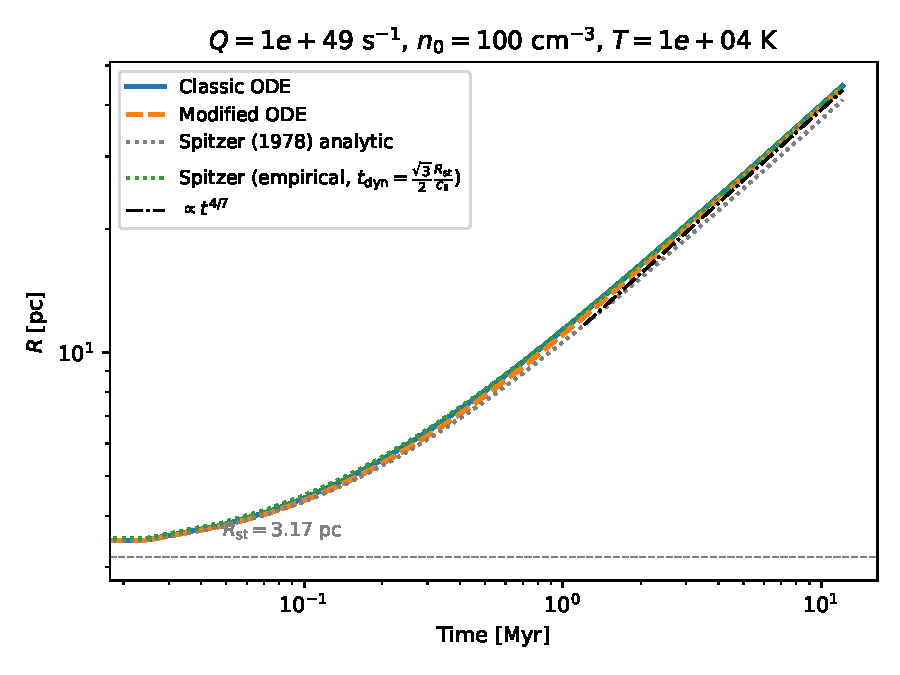
\includegraphics[width=\linewidth]{../figures/constant_density.pdf}
  \caption{HII region expansion in a uniform medium ($n_0=100$ cm$^{-3}$).
    Blue solid: classic thin-shell ODE; orange dashed: modified ODE;
    gray dotted: Spitzer (1978) analytic solution
    ($t_\mathrm{dyn}=R_\mathrm{st}/c_\mathrm{II}$);
    green dotted: empirical modification of \citet{HosokawaInutsuka2006}
    ($t_\mathrm{dyn}=\frac{\sqrt{3}}{2}R_\mathrm{st}/c_\mathrm{II}$),
    which matches the numerical solutions more closely;
    dash-dotted: $R\propto t^{4/7}$ reference slope.}
  \label{fig:constant}
\end{figure}

\subsection{Power-law density profiles}
\label{sec:results_powerlaw}

Figure~\ref{fig:powerlaw} shows the expansion for
$n(r)=n_0(r_0/r)^w$ with $w\in\{0, 0.5, 1.0, 1.4\}$.  Steeper profiles
lead to faster late-time expansion, consistent with the
$R\propto t^{4/(7-2w)}$ scaling of \citet{FrancoEtal1990}.
For $w=1.0$ the modified solution (dashed) lies \emph{above} the classic
solution at early times but \emph{below} it at late times.  This crossover
is a direct consequence of the initial zero-mass overshoot and late-time
momentum deficit described in Section~\ref{sec:crossover}.
For $w\le0.5$ the initial overpressure ($n_i/n = \sqrt{3/(3-2w)}$) is small
enough that the crossover, if present, is not visible on these axes.  For
$w=1.4$ the modified ODE is ill-conditioned at $R_\mathrm{st}$ because
$n_i \approx 3.87\,n > 2n$, so $\dot{M}_\mathrm{sh}(0) < 0$; no stable
shell forms initially and the modified solution is not shown.

\begin{figure}[ht]
  \centering
  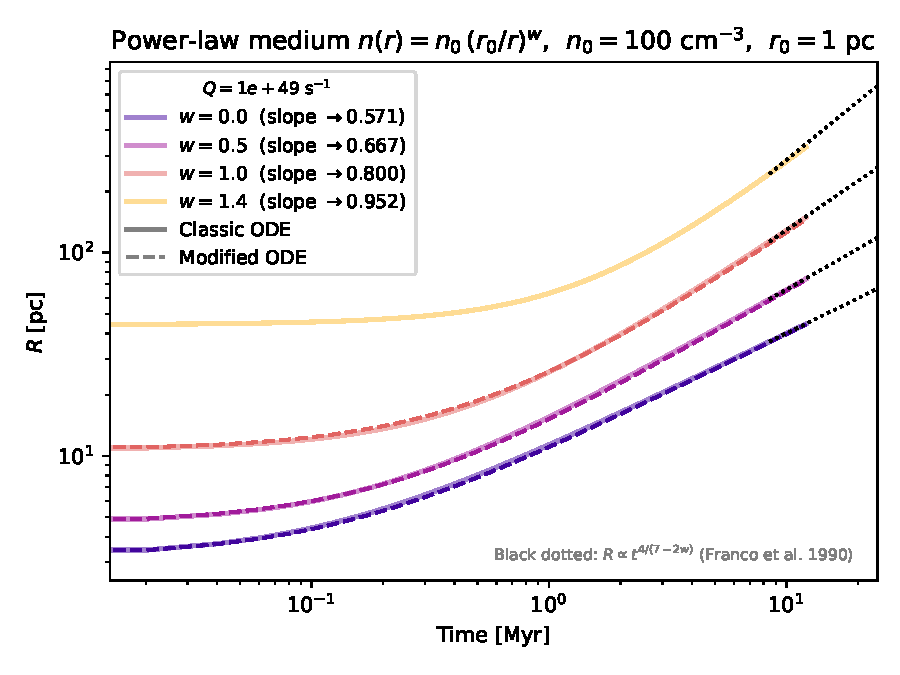
\includegraphics[width=\linewidth]{../figures/powerlaw_density.pdf}
  \caption{HII region expansion for power-law density profiles
    $n(r)=n_0(r_0/r)^w$.  Reference slopes $t^{4/(7-2w)}$ from
    \citet{FrancoEtal1990} are overlaid.}
  \label{fig:powerlaw}
\end{figure}

\subsection{Cored density profiles}
\label{sec:results_cored}

Figure~\ref{fig:cored} shows results for
$n(r)=n_0/[1+(r/r_0)^w]$ with $r_0\in\{1,5,10\}$ pc and
$w\in\{1,1.5,2\}$.  Cases with $r_0=1$ pc and $w\ge 1.5$ are
density-bounded (Table~\ref{tab:cored}) and are excluded.

\begin{figure}[ht]
  \centering
  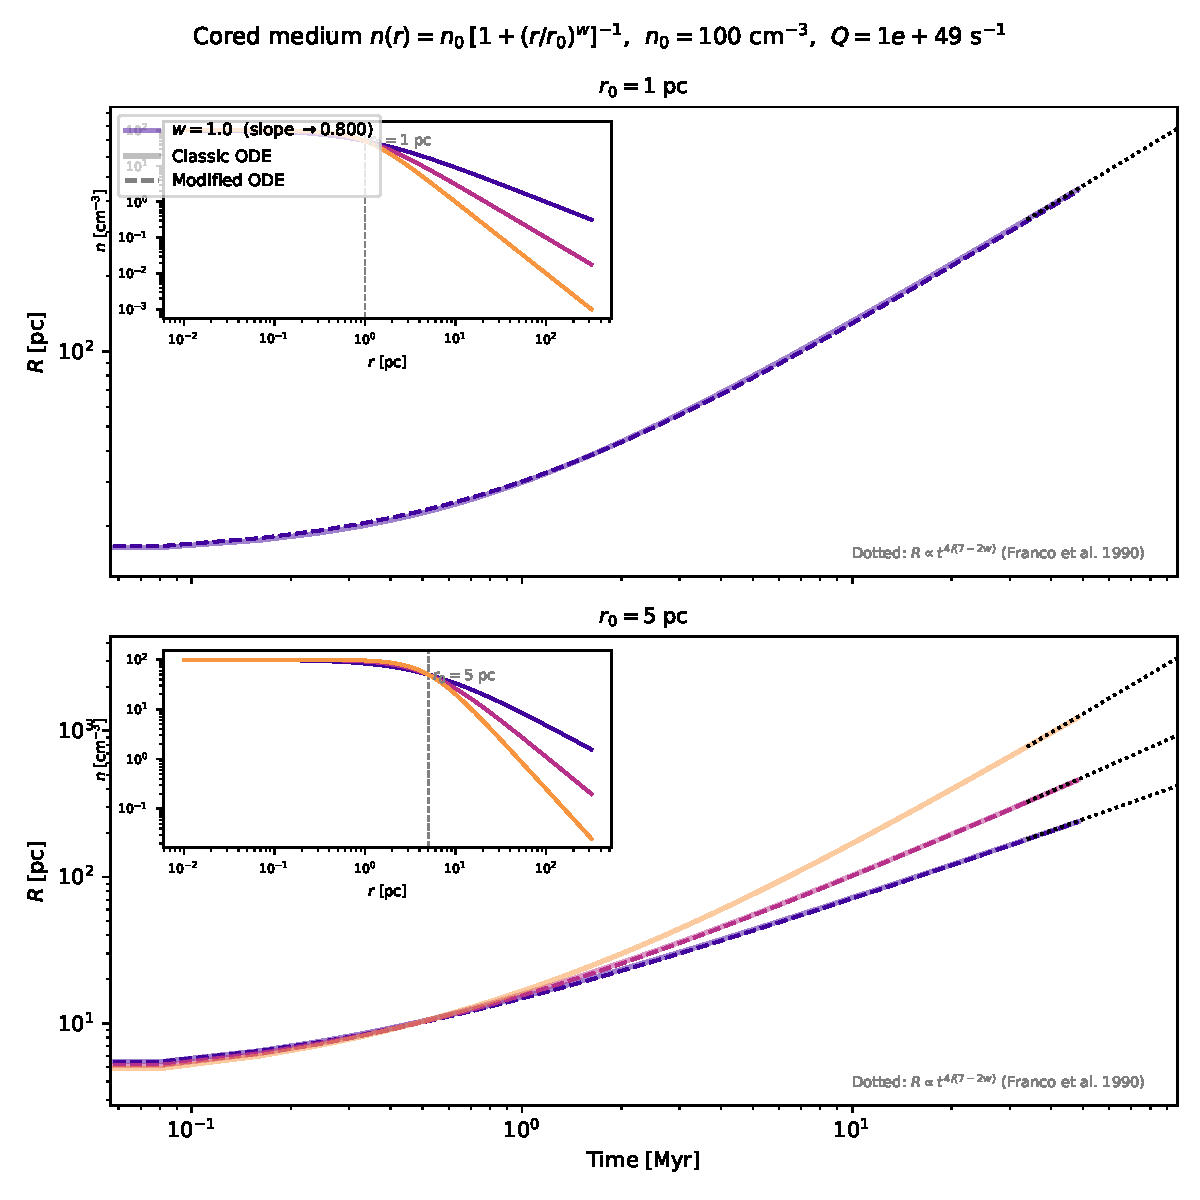
\includegraphics[width=\linewidth]{../figures/cored_density.pdf}
  \caption{HII region expansion for cored profiles
    $n(r)=n_0/[1+(r/r_0)^w]$.  Density-bounded cases are annotated.}
  \label{fig:cored}
\end{figure}

\subsection{Classic vs.\ modified Spitzer solution}
\label{sec:results_comparison}

Figure~\ref{fig:comparison} compares the classic and modified ODE systems
for uniform density over $50\,T_\mathrm{dyn}$, each with two initial
conditions: the D-critical condition $v_0=c_\mathrm{II}$ and the static
condition $v_0=0$.  The top panel shows $R(t)$: the D-critical and static
cases converge to the same $t^{4/7}$ power law at late times, but the $v_0=0$
shells expand more slowly at early times.  The middle panel shows $v(t)$: the
$v_0=0$ cases accelerate from rest, reach a peak below $c_\mathrm{II}$, then
join the decelerating power law.  The bottom panel shows
$M_\mathrm{sh}(t)$: the classic ODE initialises with the full Stromgren
mass regardless of $v_0$; the modified ODE starts from near-zero shell mass in
both cases, reflecting that the Stromgren gas is already ionized.  At late
times all four curves converge, confirming that the asymptotic evolution is
insensitive to both the initial velocity and the shell-mass formulation.

\begin{figure}[ht]
  \centering
  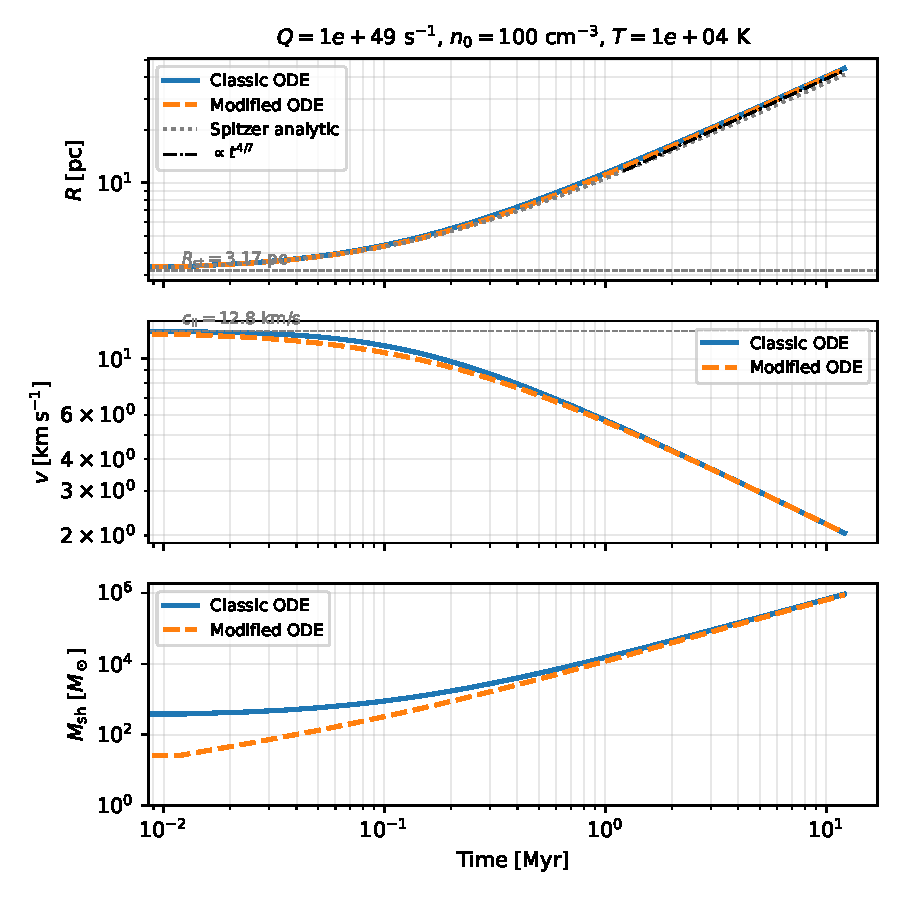
\includegraphics[width=\linewidth]{../figures/classic_vs_modified.pdf}
  \caption{Classic (blue) and modified (orange) thin-shell ODE solutions for
    uniform density, with D-critical initial velocity $v_0=c_\mathrm{II}$
    (solid) and static initial velocity $v_0=0$ (dashed).
    Top to bottom: shell radius $R(t)$, shell velocity $v(t)$, shell
    mass $M_\mathrm{sh}(t)$.  All four solutions converge to the same
    $t^{4/7}$ power law at late times.  The shell mass in the modified
    ODE is lower throughout, reflecting the zero initial shell mass and
    continuous mass transfer to the ionized interior.}
  \label{fig:comparison}
\end{figure}

%-----------------------------------------------------------------------
\section{Conclusions}
\label{sec:conclusions}
%-----------------------------------------------------------------------

We have derived the equations governing HII region expansion from first
principles and implemented them in the \texttt{hii-expansion} Python package.
The key results are:
\begin{itemize}
  \item The Str\"omgren radius is given analytically for uniform density
    (Equation~\ref{eq:Rst_uniform}) and numerically for arbitrary profiles
    (Equation~\ref{eq:Rst_numeric}).
  \item The classic Spitzer thin-shell ODE reproduces the $R\propto t^{4/7}$
    analytic solution (Equation~\ref{eq:spitzer}) within $\sim7\%$ at late
    times; the offset arises from the inertial term $M_\mathrm{sh}\dot{v}$
    retained in the ODE but neglected in the quasi-static derivation.
  \item The modified ODE (Equations~\ref{eq:ode_mod}--\ref{eq:dMsh_mod})
    correctly initializes with zero shell mass and accounts for continuous
    mass exchange at the ionization front, yielding a lower shell mass while
    leaving $R(t)$ and $v(t)$ nearly unchanged.
  \item Power-law profiles $n\propto r^{-w}$ accelerate the late-time
    expansion to $R\propto t^{4/(7-2w)}$ for $w<3/2$.
\end{itemize}

%-----------------------------------------------------------------------
\bibliography{hii_expansion}
%-----------------------------------------------------------------------

\end{document}
